\documentclass[a4paper,12pt]{article}

\usepackage{amsmath, amssymb, amsthm}
\usepackage{geometry}
\geometry{margin=1in}
\usepackage{graphicx}
\usepackage{hyperref}
\usepackage{xcolor}
\usepackage{enumitem}
\usepackage{listings}
\usepackage{float}
\usepackage{array}
\usepackage{placeins}
\usepackage{enumitem}
\usepackage{listings}
\usepackage{tikz}
\usepackage{amsmath}    
\usepackage{booktabs}
\usepackage{tabularx}


\title{Linear Regression}
\author{Christian Darvin}
\date{\today}

\begin{document}

\maketitle

\section*{Linear Regression}
A statistical technique used to find the relationship between \textbf{features} and a \textbf{label}. Possible correlations: \textbf{Positive, Negative, Non-linear, No Correlation}.
\begin{figure}[h]
    \centering
    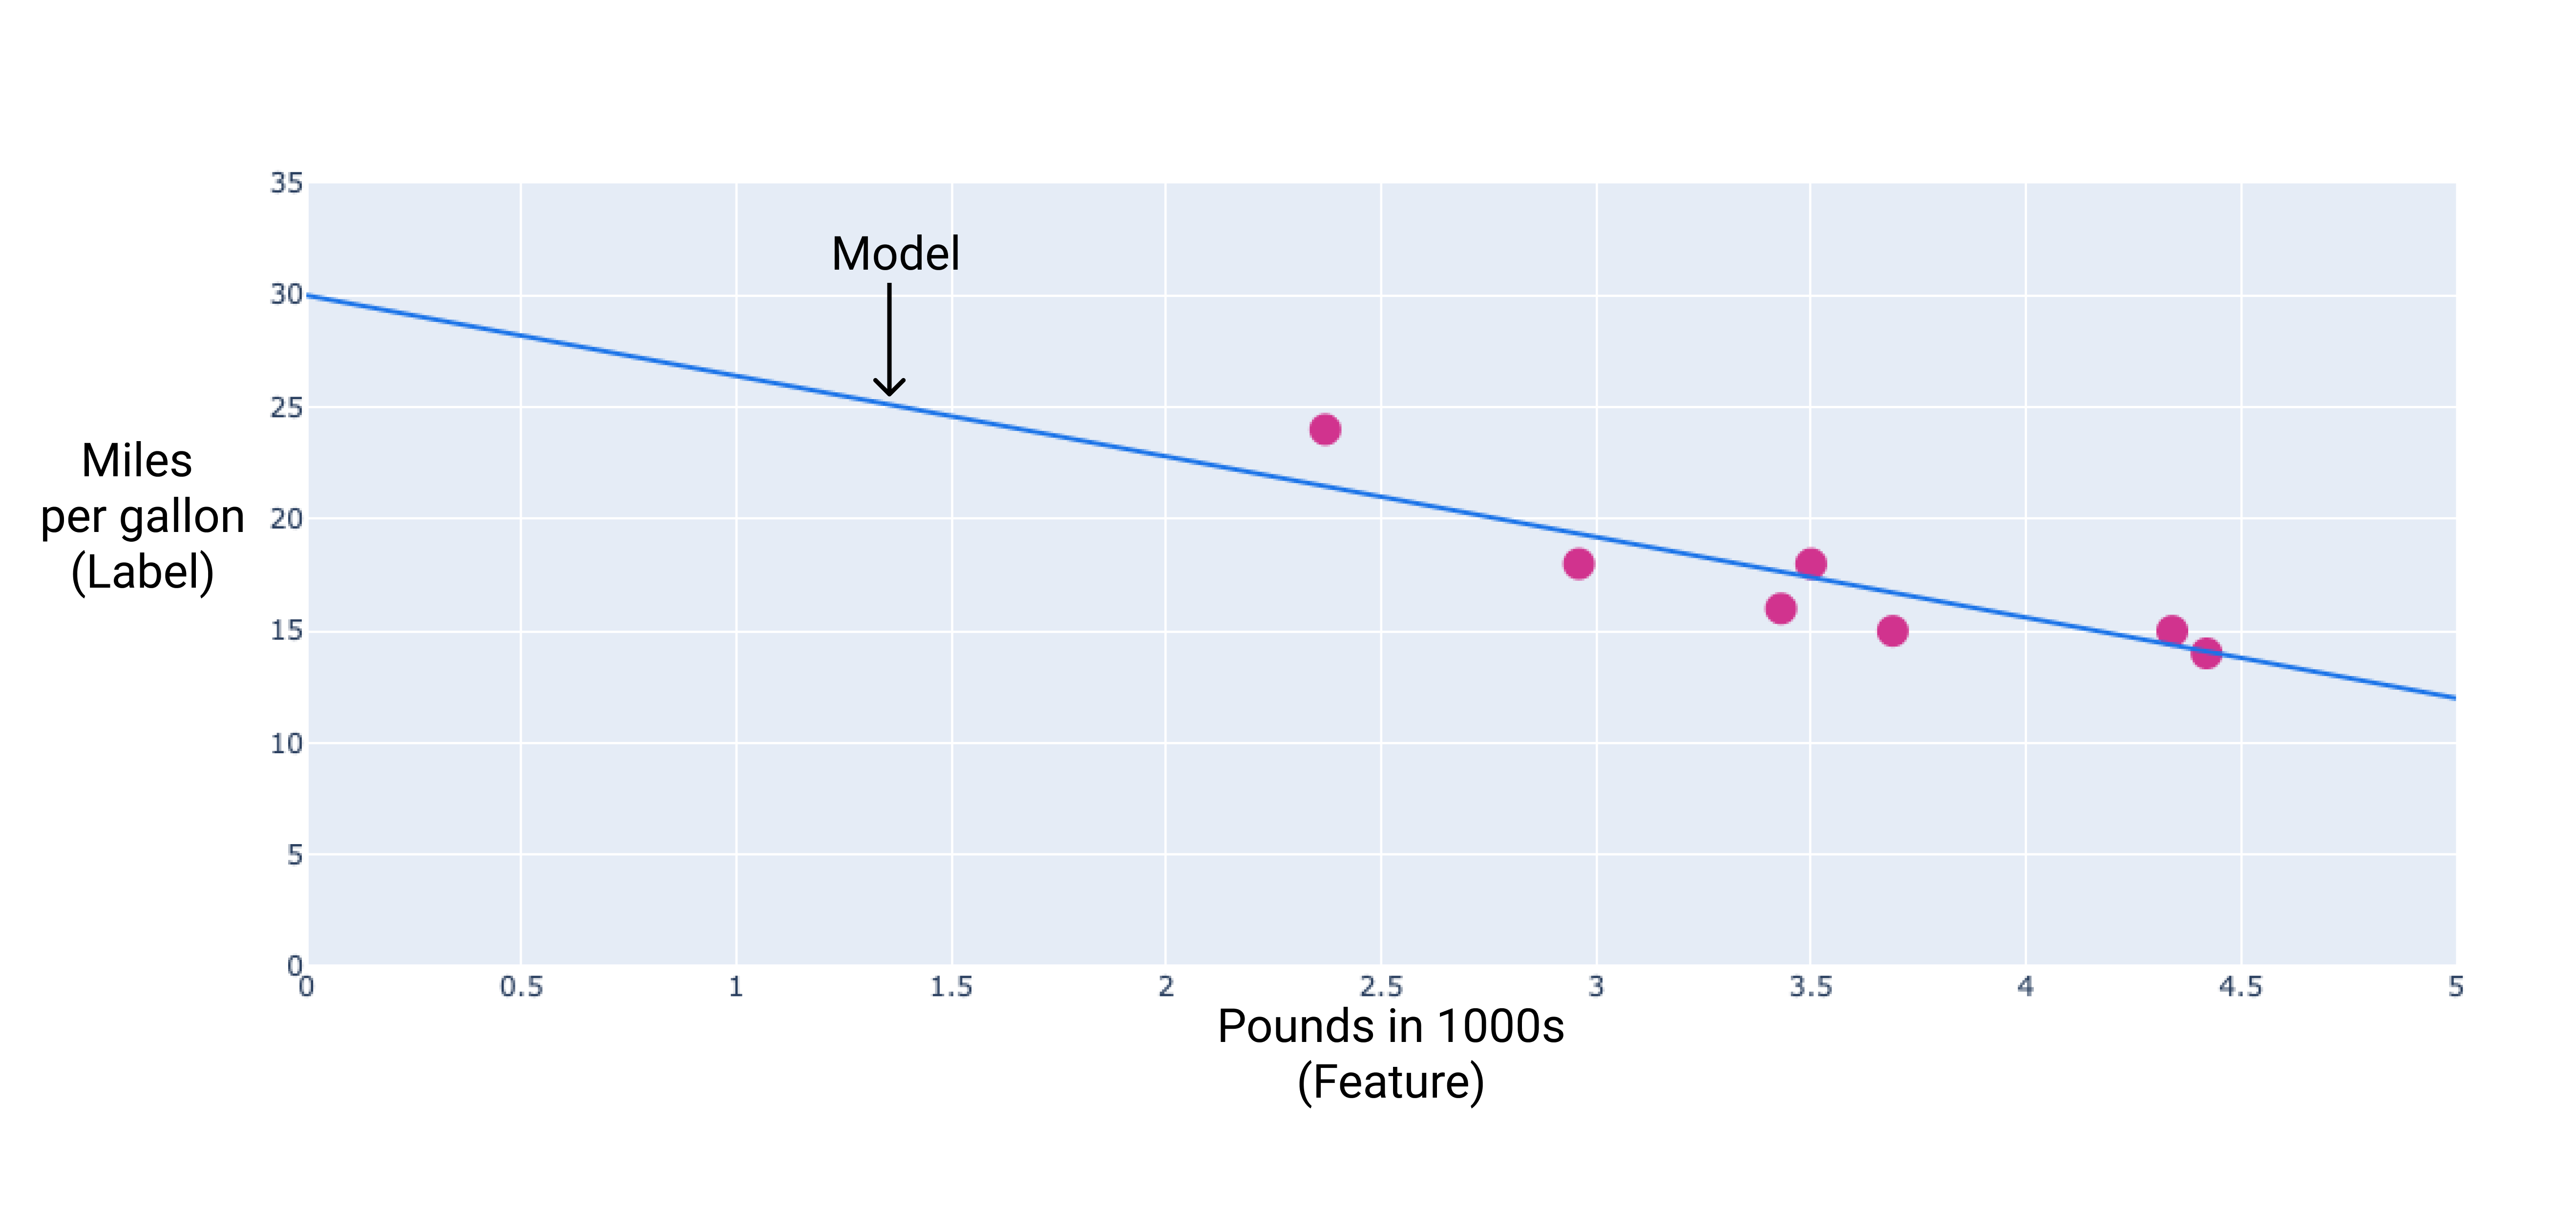
\includegraphics[width=0.7\textwidth]{../Images/linear-regression-plot.png}
    \caption{Linear Regression Plot}
    \label{fig:linear-regression-plot}
\end{figure}

\subsection*{Linear Regression Equation}

\begin{equation}
\hat{y} = b + w_1 x_1
\end{equation}

\noindent where:

$\hat{y}$: predicted label (output)

$b$: bias/parameter is the same concept as the y-intercept in algebra
 
$w_1$: weight/parameter is the same concept as slope $m$ in algebra

$x_1$: feature (input) \newline

\noindent During training, the model calculates the $w_1$ and $b$ that produce the best model.

\subsection*{Models with Multiple Features}
\begin{equation}
\hat{y} = b + w_1 x_1 + w_2 x_2 + \dots + w_n x_n
\end{equation}

\noindent $x_1, \dots, x_5$ = \{Pounds, Displacement, Acceleration, Number of Cylinders, Horsepower\}

\begin{figure}[h]
    \centering
    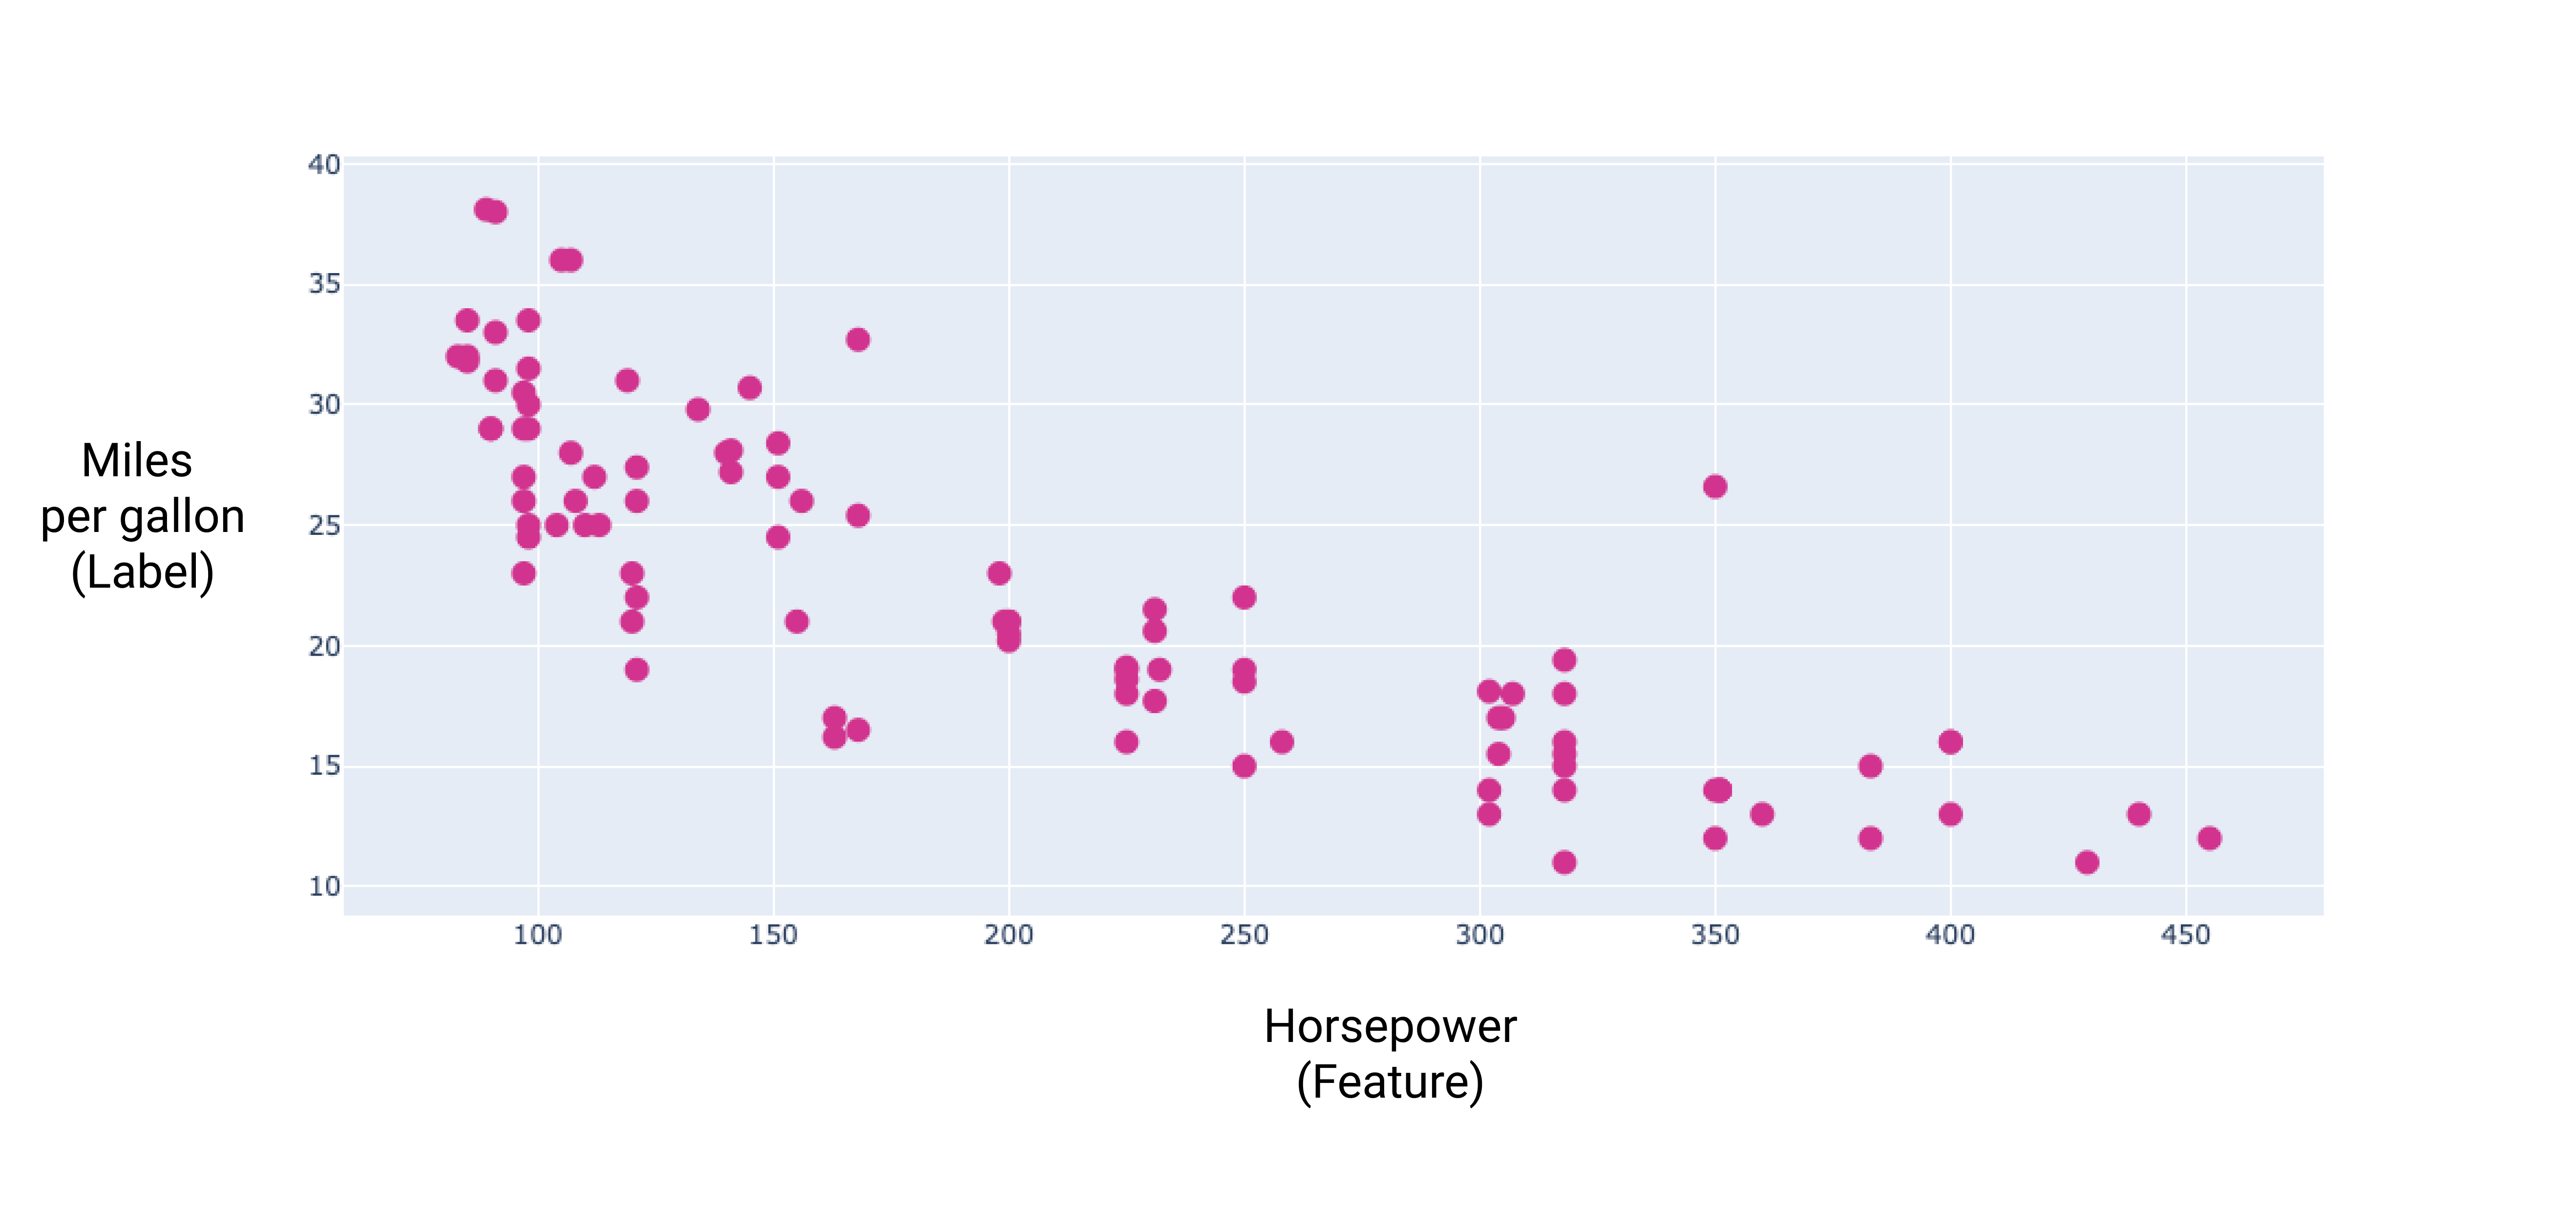
\includegraphics[width=0.7\textwidth]{../Images/horsepower-plot.png}
    \caption{Horsepower Plot}
    \label{fig:horsepower-plot}
\end{figure}

\section*{Loss Function}
A metric that describes how wrong a model's predictions are. It measures the distance between the model's predictions and the actual values. The objective is to minimize the loss, making it to its lowest possible value.

\begin{figure}[h]
    \centering
    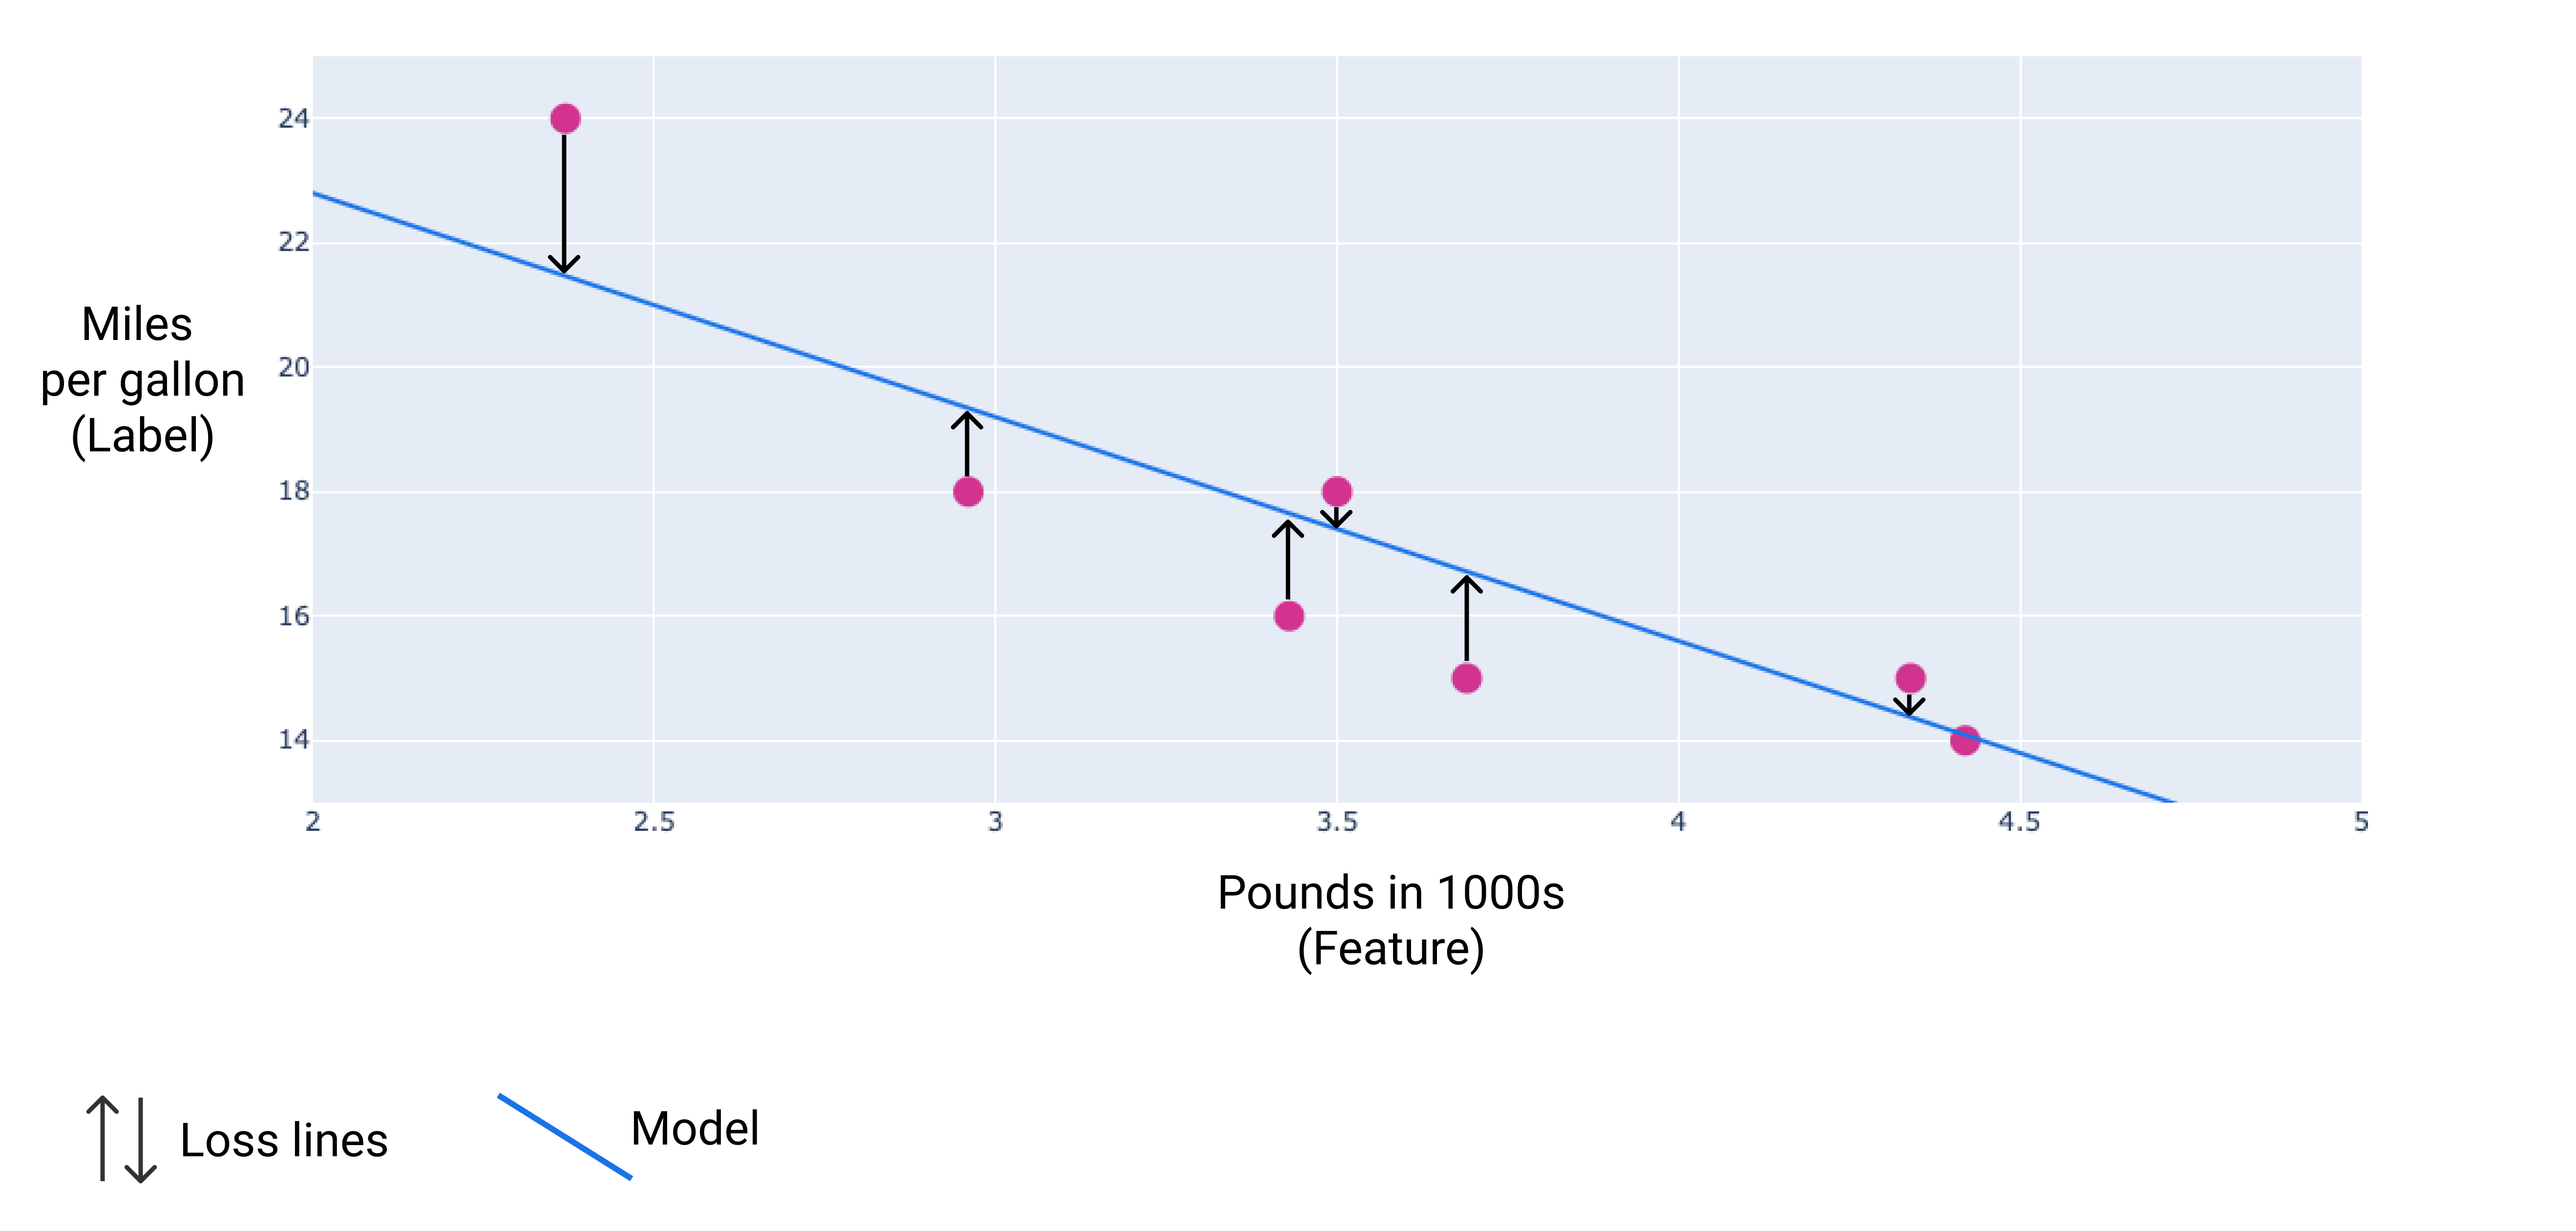
\includegraphics[width=0.7\textwidth]{../Images/loss-lines.png}
    \caption{Loss Lines}
    \label{fig:loss-lines}
\end{figure}

\subsection*{Distance of Loss}
Loss focuses on the distance, not the value. If the difference is a negative value, we need to remove the sign.

\noindent Common methods to remove the sign: 
\begin{itemize}
    \item Get the absolute value of the difference of errors
    \item Square the difference of errors
\end{itemize}

\subsection*{Error}
The difference between the actual and predicted values
\begin{equation}
error = y - \hat{y}
\end{equation}

\subsection*{Types of Loss}
\begin{center}
\begin{tabularx}{\textwidth}{@{}lXl@{}}
\toprule
Loss Type & Definition & Equation ($y$) \\ 
\midrule
$L_1$ loss & Sum of the absolute values of the errors & $\sum |y - \hat{y}|$ \\
$L_2$ loss & Sum of the squared difference of the errors & $\sum (y - \hat{y})^2$ \\
Mean Absolute Error & Average of $L_1$ losses across $N$ & $ \frac{1}{N} \sum |y - \hat{y}|$ \\
Mean Squared Error & Average of $L_2$ losses across $N$ & $ \frac{1}{N} \sum (y - \hat{y})^2$ \\
\bottomrule
\end{tabularx}
\end{center}

\noindent It is recommended to use MAE or MSE.


\section*{Gradient Descent}

\section*{Hyperparameters}


\section*{References}
\begin{itemize}
    \item \href{https://developers.google.com/machine-learning/crash-course/linear-regression}{Linear Regression - Google Developers}
    \item \href{https://developers.google.com/machine-learning/glossary}{Machine Learning Glossary - Google Developers}
\end{itemize}


\end{document}